\begin{figure}[H]
    \centering
    \makebox[\textwidth][c]{
        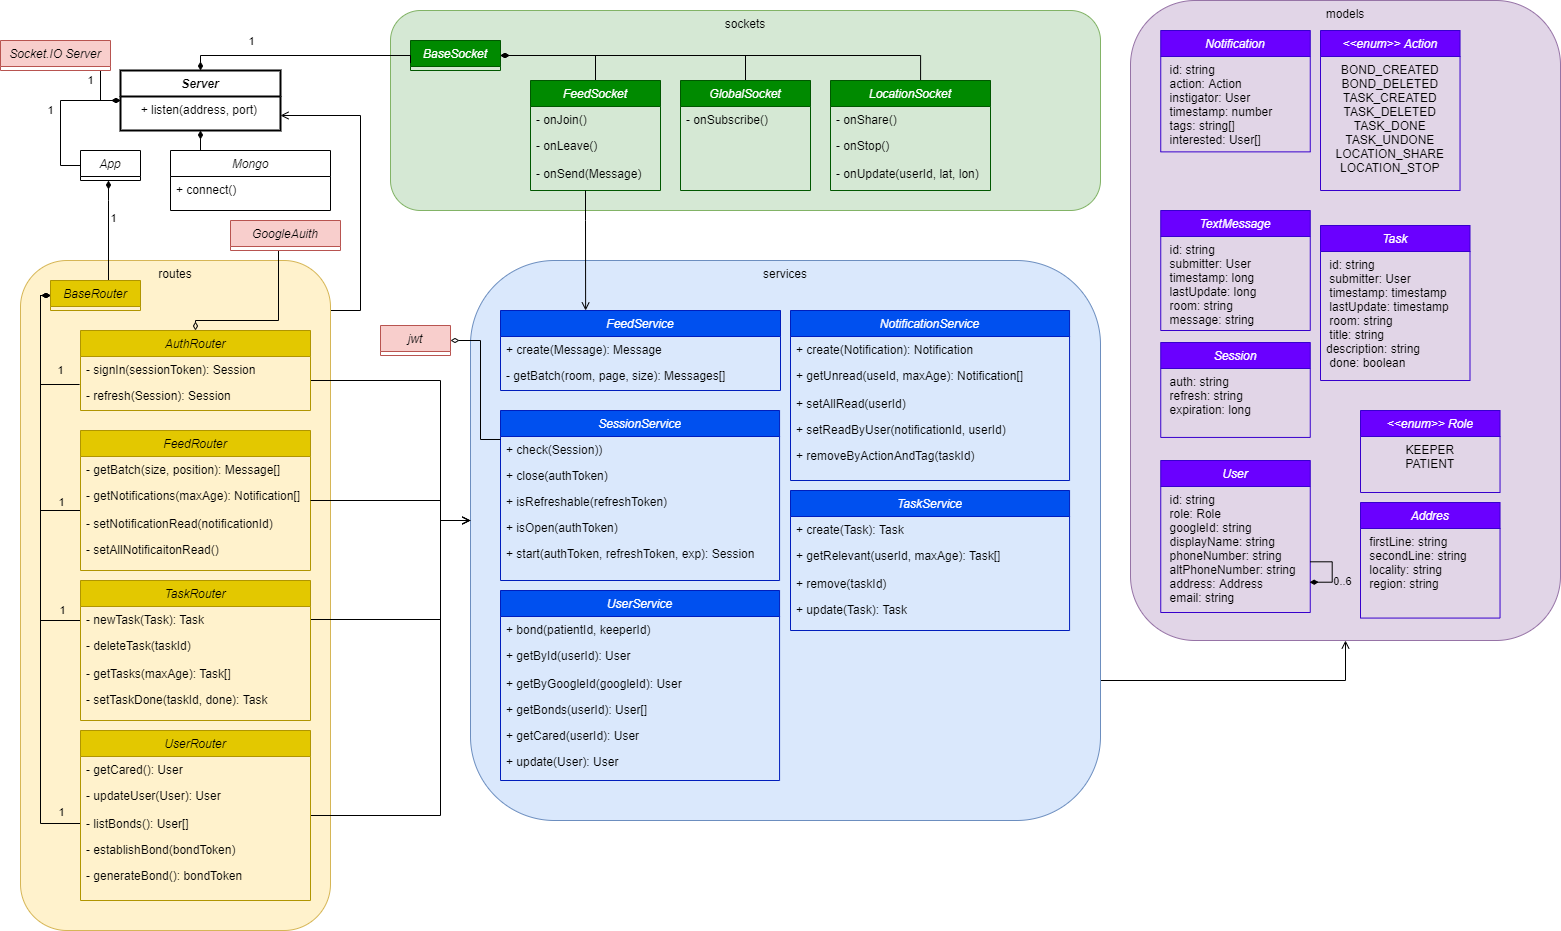
\includegraphics[width=1.2\textwidth]{Analisis/AnalisisDiagramaClasesAPI.drawio.png}
    }
    \caption{Diagrama de clases de la API}
    \label{fig:diagrama_clases_api}
\end{figure}

\section{Clases de la API}

El conjunto de clases general de la API a desarrollar se encuentra resumido en el diagrama de la \ref{fig:diagrama_clases_api}. En el caso de la API los distinto módulos representarán no clases sino paquetes de funciones servidos por sus diferentes índices. Salvo en el caso del paquete de modelos que estará conformado por clases. Los módulos en rojo corresponden a librerías externas ya identificadas.

\subsection{Root}

\begin{longtable}{|p{0.25\textwidth} p{0.75\textwidth}|}
    \hline
    \multicolumn{2}{|l|}{Server} \\ \hline \hline
    Descripción      & Módulo principal y global del sistema. Inicializa todos los sistemas de la API en su lanzamiento desde el punto de entrada de la aplicación \\ \hline
    \multicolumn{2}{|l|}{Funciones} \\
    \emph{listen}  & Despliega el servidor en la direcciones y puerto especificados  \\ \hline
    \caption{Especificación de la clase Server}
    \label{class:api:server}
\end{longtable}

\begin{longtable}{|p{0.25\textwidth} p{0.75\textwidth}|}
    \hline
    \multicolumn{2}{|l|}{App} \\ \hline \hline
    Descripción      & Implementación del servidor Express, punto de entrada de las consultas REST \\ \hline
    \caption{Especificación de la clase App}
    \label{class:api:app}
\end{longtable}

\vspace{-20pt}
\begin{longtable}{|p{0.25\textwidth} p{0.75\textwidth}|}
    \hline
    \multicolumn{2}{|l|}{Mongo} \\ \hline \hline
    Descripción      & Módulo a cargo de la lógica relativa a la conexión de Mongoose con la base de datos \\ \hline
    \multicolumn{2}{|l|}{Funciones} \\
    \emph{connect}  & Crea la conexión con la base de datos remota  \\ \hline
    \caption{Especificación de la clase Mongo}
    \label{class:api:mongo}
\end{longtable}

\vspace{-20pt}
\subsection{Routes}

\begin{longtable}{|p{0.25\textwidth} p{0.75\textwidth}|}
    \hline
    \multicolumn{2}{|l|}{BaseRouter} \\ \hline \hline
    Descripción      & Manejador raíz encargado de redireccionar las peticiones REST al manejador encargado de cada una según la ruta \\ \hline
    \caption{Especificación de la clase BaseRouter}
    \label{class:api:base_router}
\end{longtable}

\vspace{-20pt}
\begin{longtable}{|p{0.25\textwidth} p{0.75\textwidth}|}
    \hline
    \multicolumn{2}{|l|}{AuthRouter} \\ \hline \hline
    Descripción      & Manejador de las peticiones de /auth \\ \hline
    \multicolumn{2}{|l|}{Funciones} \\
    \emph{signIn}  & Crea una sesión para el usuario  \\ 
    \emph{signIn}  & Refresca la sesión del usuario  \\ \hline
    \caption{Especificación de la clase AuthRouter}
    \label{class:api:auth_router}
\end{longtable}

\vspace{-20pt}
\begin{longtable}{|p{0.3\textwidth} p{0.7\textwidth}|}
    \hline
    \multicolumn{2}{|l|}{FeedRouter} \\ \hline \hline
    Descripción      & Manejador de las peticiones de /feed \\ \hline
    \multicolumn{2}{|l|}{Funciones} \\
    \emph{getBatch}  & Devuelve el conjunto de mensajes solicitado por el usuario  \\ 
    \emph{getNotifications}  & Devuelve las notificaciones pendientes del usuario  \\ 
    \emph{setNotificationRead}  & Marcar una notificación como leída  \\ 
    \emph{setAllNotificationsRead}  & Marca todas las notificaciones del usuario como leídas  \\ \hline
    \caption{Especificación de la clase FeedRouter}
    \label{class:api:feed_router}
\end{longtable}

\begin{figure}[H]
\begin{longtable}{|p{0.25\textwidth} p{0.75\textwidth}|}
    \hline
    \multicolumn{2}{|l|}{TaskRouter} \\ \hline \hline
    Descripción      & Manejador de las peticiones de /task \\ \hline
    \multicolumn{2}{|l|}{Funciones} \\
    \emph{newTask}  & Crea una nueva tarea  \\ 
    \emph{deleteTask}  & Elimina la tarea especificada  \\ 
    \emph{getTasks}  & Retorna las tareas relevantes relacionadas con el usuario  \\ 
    \emph{setTaskDone}  & Marca una tarea como hecha/no hecha  \\ \hline
    \caption{Especificación de la clase TaskRouter}
    \label{class:api:task_router}
\end{longtable}
\end{figure}

\vspace{-20pt}
\begin{longtable}{|p{0.25\textwidth} p{0.75\textwidth}|}
    \hline
    \multicolumn{2}{|l|}{UserRouter} \\ \hline \hline
    Descripción      & Manejador de las peticiones de /user \\ \hline
    \multicolumn{2}{|l|}{Funciones} \\
    \emph{getCared}  & Devuelve paciente vinculado con el usuario  \\
    \emph{updateUser}  & Actualiza la información del usuario  \\
    \emph{listBonds}  & Devuelve los vínculos del usuario  \\
    \emph{establishBond}  & Crea un vínculo entre usuarios  \\
    \emph{generateBond}  & Genera un código de vinculación  \\ \hline
    \caption{Especificación de la clase UserRouter}
    \label{class:api:user_router}
\end{longtable}

\vspace{-30pt}
\subsection{Sockets}

\begin{longtable}{|p{0.25\textwidth} p{0.75\textwidth}|}
    \hline
    \multicolumn{2}{|l|}{BaseSocket} \\ \hline \hline
    Descripción      & Manejador raíz encargado de redireccionar los eventos del WebSocket al manejador encargado de cada una según la sala \\ \hline
    \caption{Especificación de la clase BaseSocket}
    \label{class:api:base_socket}
\end{longtable}

\vspace{-20pt}
\begin{longtable}{|p{0.25\textwidth} p{0.75\textwidth}|}
    \hline
    \multicolumn{2}{|l|}{FeedSocket} \\ \hline \hline
    Descripción      & Manejador de la sala del Feed \\ \hline
    \multicolumn{2}{|l|}{Funciones} \\
    \emph{onJoin}  & Gestiona la entrada de un usuario en la sala  \\
    \emph{onLeave}  & Gestione el abandono de la sala de un usuario  \\
    \emph{onSendMessage}  & Maneja el envío de un mensaje  \\ \hline
    \caption{Especificación de la clase FeedSocket}
    \label{class:api:feed_socket}
\end{longtable}

\newpage
\begin{longtable}{|p{0.25\textwidth} p{0.75\textwidth}|}
    \hline
    \multicolumn{2}{|l|}{GlobalSocket} \\ \hline \hline
    Descripción      & Manejador de la sala global \\ \hline
    \multicolumn{2}{|l|}{Funciones} \\
    \emph{onSubscribe}  & Gestiona la suscripción de un usuario a la sala \\ \hline
    \caption{Especificación de la clase GlobalSocket}
    \label{class:api:global_socket}
\end{longtable}

\begin{longtable}{|p{0.25\textwidth} p{0.75\textwidth}|}
    \hline
    \multicolumn{2}{|l|}{LocationSocket} \\ \hline \hline
    Descripción      & Manejador de la sala de la geolocalización \\ \hline
    \multicolumn{2}{|l|}{Funciones} \\
    \emph{onShare}  & Gestiona la entrada de un usuario en la sala  \\
    \emph{onStop}  & Gestione el abandono de la sala de un usuario  \\
    \emph{onUpdate}  & Maneja el envío de una localización  \\ \hline
    \caption{Especificación de la clase LocationSocket}
    \label{class:api:location_socket}
\end{longtable}

\subsection{Services}

\begin{longtable}{|p{0.25\textwidth} p{0.75\textwidth}|}
    \hline
    \multicolumn{2}{|l|}{FeedService} \\ \hline \hline
    Descripción      & Servicio a cargo de los mensajes del feed \\ \hline
    \multicolumn{2}{|l|}{Funciones} \\
    \emph{create}  & Crea y persiste un nuevo mensaje  \\
    \emph{getBatch}  & Devuelve la lista de mensajes especificada  \\ \hline
    \caption{Especificación de la clase FeedService de la API}
    \label{class:api:feed_service}
\end{longtable}

\begin{longtable}{|p{0.3\textwidth} p{0.7\textwidth}|}
    \hline
    \multicolumn{2}{|l|}{NotificationService} \\ \hline \hline
    Descripción      & Servicio a cargo de las notificaciones \\ \hline
    \multicolumn{2}{|l|}{Funciones} \\
    \emph{create}  & Crea y persiste una nueva notificación  \\
    \emph{getUnread}  & Devuelve la lista de notificaciones no leídas de un usuario  \\
    \emph{setAllRead}  & Marca todas las notificaciones de un usuario como leídas  \\
    \emph{setReadByUser}  & Marca una notificación como leída  \\
    \emph{removeByActionAndTag}  & Elimina las notificaciones que tienen la misma acción y etiquetas  \\ \hline
    \caption{Especificación de la clase NotificationService}
    \label{class:api:notification_service}
\end{longtable}

\begin{longtable}{|p{0.25\textwidth} p{0.75\textwidth}|}
    \hline
    \multicolumn{2}{|l|}{SessionService} \\ \hline \hline
    Descripción      & Servicio a cargo de las sesiones de usuario \\ \hline
    \multicolumn{2}{|l|}{Funciones} \\
    \emph{check}  & Comprueba la validez de una sesión  \\
    \emph{close}  & Cierra la sesión especificada  \\
    \emph{isRefreshable}  & Comprueba si una sesión se puede refrescar  \\
    \emph{isOpen}  & Comprueba si una sesión está activa  \\
    \emph{start}  & Crea una nueva sesión de usuario  \\ \hline
    \caption{Especificación de la clase SessionService}
    \label{class:api:session_service}
\end{longtable}

\begin{longtable}{|p{0.25\textwidth} p{0.75\textwidth}|}
    \hline
    \multicolumn{2}{|l|}{TaskService} \\ \hline \hline
    Descripción      & Servicio a cargo de las tareas \\ \hline
    \multicolumn{2}{|l|}{Funciones} \\
    \emph{create}  & Crea y persiste una nueva tarea  \\
    \emph{getRelevant}  & Devuelve la lista de tareas relevantes de un usuario  \\
    \emph{remove}  & Elimina la tarea especificada  \\
    \emph{update}  & Actualiza una tarea  \\ \hline
    \caption{Especificación de la clase TaskService de la API}
    \label{class:api:task_service}
\end{longtable}

\begin{longtable}{|p{0.25\textwidth} p{0.75\textwidth}|}
    \hline
    \multicolumn{2}{|l|}{UserService} \\ \hline \hline
    Descripción      & Servicio a cargo de los datos de usuario \\ \hline
    \multicolumn{2}{|l|}{Funciones} \\
    \emph{bond}  & Crea un vínculo entre usuarios  \\
    \emph{getById}  & Retorna el usuario con la identidad especificada  \\
    \emph{getByGoogleId}  & Retorna el usuario con la identidad de Google especificada  \\
    \emph{getBonds}  & Devuelve los vínculos de un usuario  \\
    \emph{getCared}  & Devuelve el paciente vinculado de un usuario  \\
    \emph{update}  & Actualiza los datos de un usuario  \\ \hline
    \caption{Especificación de la clase UserService de la API}
    \label{class:api:user_service}
\end{longtable}

\newpage
\subsection{Models}

\begin{longtable}{|p{0.25\textwidth} p{0.75\textwidth}|}
    \hline
    \multicolumn{2}{|l|}{Action} \\ \hline \hline
    Descripción      & Lista de posibles acciones notificables \\ \hline
    \multicolumn{2}{|l|}{Valores} \\
    \emph{BOND CREATED}  & Creación de un vínculo  \\
    \emph{BOND DELETED}  & Eliminación de un vínculo  \\
    \emph{TASK CREATED}  & Creación de una tarea  \\
    \emph{TASK DELETED}  & Eliminación de una tarea  \\
    \emph{TASK DONE}  & Actualización de una tarea a hecha  \\
    \emph{TASK UNDONE}  & Actualización de una tarea a no hecha  \\
    \emph{LOCATION SHARE}  & Ubicación empezando a ser compartida  \\
    \emph{LOCATION STOP}  & Ubicación dejando de ser compartida  \\ \hline
    \caption{Especificación de la clase Action de la API}
    \label{class:api:action}
\end{longtable}

\begin{longtable}{|p{0.25\textwidth} p{0.75\textwidth}|}
    \hline
    \multicolumn{2}{|l|}{Address} \\ \hline \hline
    Descripción      & Abstracción de direcciones postales \\ \hline
    \multicolumn{2}{|l|}{Propiedades} \\
    \emph{firstLine}  & Primera línea (por ejemplo, calle y número)  \\
    \emph{secondLine}  & Segunda línea (por ejemplo, piso y puerta)  \\
    \emph{locality}  & Localidad  \\
    \emph{region}  & Región (por ejemplo, provincia o estado)  \\ \hline
    \caption{Especificación de la clase Address de la API}
    \label{class:api:address}
\end{longtable}

\begin{longtable}{|p{0.25\textwidth} p{0.75\textwidth}|}
    \hline
    \multicolumn{2}{|l|}{Notification} \\ \hline \hline
    Descripción      & Entidad representante de las notificaciones de la aplicación \\ \hline
    \multicolumn{2}{|l|}{Propiedades} \\
    \emph{id}  & ID  \\
    \emph{action}  & Acción a notificar  \\
    \emph{instigator}  & Autor de la acción  \\
    \emph{timestamp}  & Instante de realización de la acción  \\
    \emph{tags}  & Etiquetas con información extra de la notificación  \\
    \emph{interested}  & Lista de usuarios receptores de la notificación  \\ \hline
    \caption{Especificación de la clase Notification de la API}
    \label{class:api:notification}
\end{longtable}

\begin{longtable}{|p{0.25\textwidth} p{0.75\textwidth}|}
    \hline
    \multicolumn{2}{|l|}{Role} \\ \hline \hline
    Descripción      & Lista de posibles roles de los usuarios \\ \hline
    \multicolumn{2}{|l|}{Valores} \\
    \emph{PATIENT}  & Pacientes  \\
    \emph{KEEPER}  & Cuidadores  \\ \hline
    \caption{Especificación de la clase Role de la API}
    \label{class:api:role}
\end{longtable}

\begin{longtable}{|p{0.25\textwidth} p{0.75\textwidth}|}
    \hline
    \multicolumn{2}{|l|}{Session} \\ \hline \hline
    Descripción      & Entidad representante de una sesión de usuario \\ \hline
    \multicolumn{2}{|l|}{Propiedades} \\
    \emph{auth}  & Token de autenticación de la sesión  \\
    \emph{refresh}  & Token de refresco de la sesión  \\
    \emph{expiration}  & Instante de expiración de la sesión  \\ \hline
    \caption{Especificación de la clase Session de la API}
    \label{class:api:session}
\end{longtable}

\begin{longtable}{|p{0.25\textwidth} p{0.75\textwidth}|}
    \hline
    \multicolumn{2}{|l|}{Task} \\ \hline \hline
    Descripción      & Entidad representante de las notificaciones de la aplicación \\ \hline
    \multicolumn{2}{|l|}{Propiedades} \\
    \emph{id}  & ID  \\
    \emph{submitter}  & Autor de la tarea  \\
    \emph{timestamp}  & Instante de envío de la tarea \\
    \emph{lastUpdate}  & Última actualización de la tarea  \\
    \emph{room}  & Sala de envío de la tarea  \\
    \emph{title}  & Título  \\
    \emph{description}  & Descripción  \\
    \emph{done}  & Estado: hecha/no hecha  \\ \hline
    \caption{Especificación de la clase Task de la API}
    \label{class:api:task}
\end{longtable}

\newpage
\begin{longtable}{|p{0.25\textwidth} p{0.75\textwidth}|}
    \hline
    \multicolumn{2}{|l|}{TextMessage} \\ \hline \hline
    Descripción      & Entidad representante de los mensajes de texto del Feed \\ \hline
    \multicolumn{2}{|l|}{Propiedades} \\
    \emph{id}  & ID  \\
    \emph{submitter}  & Autor del mensaje  \\
    \emph{timestamp}  & Instante de envío del mensaje \\
    \emph{lastUpdate}  & Última actualización del mensaje  \\
    \emph{room}  & Sala de envío del mensaje  \\
    \emph{message}  & Mensaje enviado  \\ \hline
    \caption{Especificación de la clase TextMessage de la API}
    \label{class:api:text_message}
\end{longtable}

\begin{longtable}{|p{0.25\textwidth} p{0.75\textwidth}|}
    \hline
    \multicolumn{2}{|l|}{User} \\ \hline \hline
    Descripción      & Entidad representante de los usuarios de la aplicación \\ \hline
    \multicolumn{2}{|l|}{Propiedades} \\
    \emph{id}  & ID  \\
    \emph{role}  & Rol  \\
    \emph{googleId}  & Identidad de Google  \\
    \emph{displayName}  & Nombre para mostrar al resto de usuarios  \\
    \emph{phoneNumber}  & Teléfono principal  \\
    \emph{altPhoneNumber}  & Teléfono alternativo  \\
    \emph{address}  & Dirección postal  \\
    \emph{email}  & Dirección electrónica  \\
    \emph{bonds}  & Lista de usuarios vinculados  \\ \hline
    \caption{Especificación de la clase User de la API}
    \label{class:api:user}
\end{longtable}
